\documentclass[a4paper, 10pt, oneside]{article} % Ich habe "article und nicht book gewählt

\usepackage[a4paper, left=2cm, right=5cm]{geometry}
\usepackage[utf8]{inputenc}
\usepackage[ngerman]{babel}
\usepackage[T1]{fontenc}
\usepackage{graphicx}
\usepackage[svgnames]{xcolor} % Required for colour specification
\usepackage{fouriernc} % Use the New Century Schoolbook font
\usepackage{setspace}



\begin{document}

%---------------------------------------------------------------------------------------------------------------------------

\begin{titlepage}

	\newgeometry{
  	left=4cm,
 	right=4cm,
  	bindingoffset=5mm
	}

	\centering 
	
	%------------------------------------------------
	%	Doppelstrich oben
	%------------------------------------------------
	
	\rule{\textwidth}{1pt} % Dicke Linie
	
	\vspace{2pt}\vspace{-\baselineskip}
	
	\rule{\textwidth}{0.4pt} 
	
	\vspace{0.1\textheight} % Abstand zwischen Überschrift und Titel
	
	%------------------------------------------------
	%	Titel
	%------------------------------------------------
	
	\textcolor{Blue}{ % Rote Schriftfarbe
		{\Huge PaperCon}\\[0.5\baselineskip] % Erste Überschrift
		{\Large ein Projekt von}\\[0.5\baselineskip] % Zweite Überschrift
		{\Huge Ben Eric und Johannes} % Dritte Überschrift
	}
	
	\vspace{0.025\textheight} % Whitespace between the title and short horizontal rule
	
	\rule{0.3\textwidth}{0.4pt} % Short horizontal rule under the title
	
	\vspace{0.1\textheight} % Whitespace between the thin horizontal rule and the author name
	
	%------------------------------------------------
	%	Autor
	%------------------------------------------------
	
	{\Large \textsc{Dokumentation von Johannes Brandt}} % Autorenname
	
	\vfill % Lücke zwischen Autor und Datum
	
	%------------------------------------------------
	%	Datum von Projektanfang bis Projektende
	%------------------------------------------------
	
	{\large\textsc{6 Februar 2023 - 24 Februar 2023}} % Startdatum bis Enddatum
	
	\vspace{0.1\textheight} % Whitespace under the publisher text
	
	%------------------------------------------------
	%	Bottom rules
	%------------------------------------------------
	
	\rule{\textwidth}{0.4pt} % Thin horizontal rule
	
	\vspace{2pt}\vspace{-\baselineskip} % Whitespace between rules
	
	\rule{\textwidth}{1pt} % Thick horizontal rule
	
\end{titlepage}

\restoregeometry


%---------------------------------------------------------------------------------------------------------------------------



\huge{\underline{\textbf{Inhaltsverzeichnis}}}
\newline

\section{Generelle Informationen und Einleitung}
\subsection*{$\Rightarrow$ Seite 1 bis Seite 2 }
\vspace*{4mm}


\section{Arbeitstagebuch}
\subsection*{$\Rightarrow$ Von Seite 3 bis Seite 5}
\vspace*{4mm}

\section{Code-Dokumentation}
\subsection*{$\Rightarrow$ Von Seite 6 bis Seite 8}
\vspace*{4mm}

\section{Canvas}
\subsection*{$\Rightarrow$ Von Seite 6 bis Seite 8}
\vspace*{4mm}

\section{Organisatorisches}
\subsection*{$\Rightarrow$ Von Seite 6 bis Seite 8}
\vspace*{4mm}



%---------------------------------------------------------------------------------------------------------------------------

\newpage


\huge{\underline{\textbf{Einleitung}}}
\newline

\section*{Worum geht unser Projekt:}


\begin{normalsize}
\begin{spacing}{1}

Unser Projekt ist eine mit der Software BlueJ und der Bibliothek GLOOP erstellte Flugsimulation in welcher Spielende ein Flugzeug selber fliegen und steuern können. Es muss selbstständig gestartet und gelandet werden und eventuell müssen weitere Schwierigkeiten überwunden werden.

\section*{Unsere Ziele für dieses Projekt:}

\subsection*{Ist-Ziele:}

\begin{itemize}
\item[$\Rightarrow$] Eine Dokumentation (angefangen) und Canvas
\item[$\Rightarrow$] Ein sich öffnendes Spielefenster
\item[$\Rightarrow$] Ein Flugzeug mit einigen Farben und Texturen
\end{itemize}

\subsection*{Soll-Ziele:}

\begin{itemize}
\item[$\Rightarrow$] Flugzeug soll sich bewegen (fliegen) können
\item[$\Rightarrow$] Flugzeug soll starten und landen können
\item[$\Rightarrow$] Es soll eine Start und eine Landebahn geben
\end{itemize}

\subsection*{Kann-Ziele:}

\begin{itemize}
\item[$\Rightarrow$] Ergänzende Details (z.B. Flugzeug neigt sich passend)
\item[$\Rightarrow$] evtl. Terrain
\end{itemize}

\end{spacing}
\end{normalsize}

%---------------------------------------------------------------------------------------------------------------------------


%---------------------------------------------------------------------------------------------------------------------------

\newpage


\huge{\underline{\textbf{Arbeitstagebuch}}}
\newline

\section*{12. Februar 2023 - Sonntag:}


\begin{normalsize}
\begin{spacing}{1}

Heute habe ich mir vorgenommen in Paint.net ein grobes Modell von dem Flugzeug für unser Projekt zu entwerfen. Dieses soll von vier verschiedenen Ansichten zu sehen sein und relativ simpel aufgebaut damit es nicht allzu schwer zu implementieren ist. Das Ergebnis ist auf dem Bild zu sehen.

\begin{figure}[h]
 \centering
 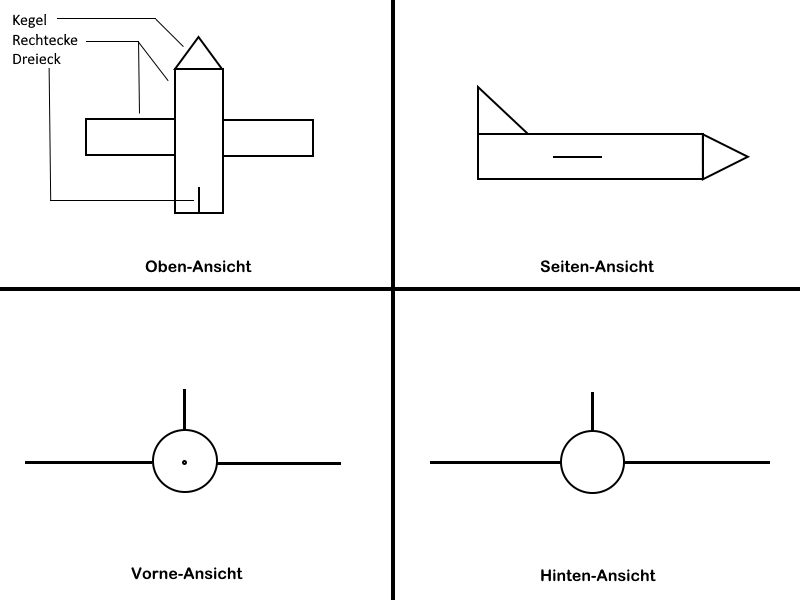
\includegraphics[width=8cm]{Bilder/Flugzeug-Entwürfe/Entwurf1.png}
 \caption{Flugzeug-Entwurf}
\end{figure}

Zusätzlich habe ich in dieser PDF das Inhaltsverzeichnis und die erste Seite eingerichtet. Die Titelseite hatte ich bereits vorher mit einer Vorlage eingerichtet. Der Link dazu ist auf der Quellenseite zu finden. Das Canva mit dem aktuellen Stand ist das 'Canva1' auf den Canva-Seiten.

%\begin{figure}[h]
%\centering
%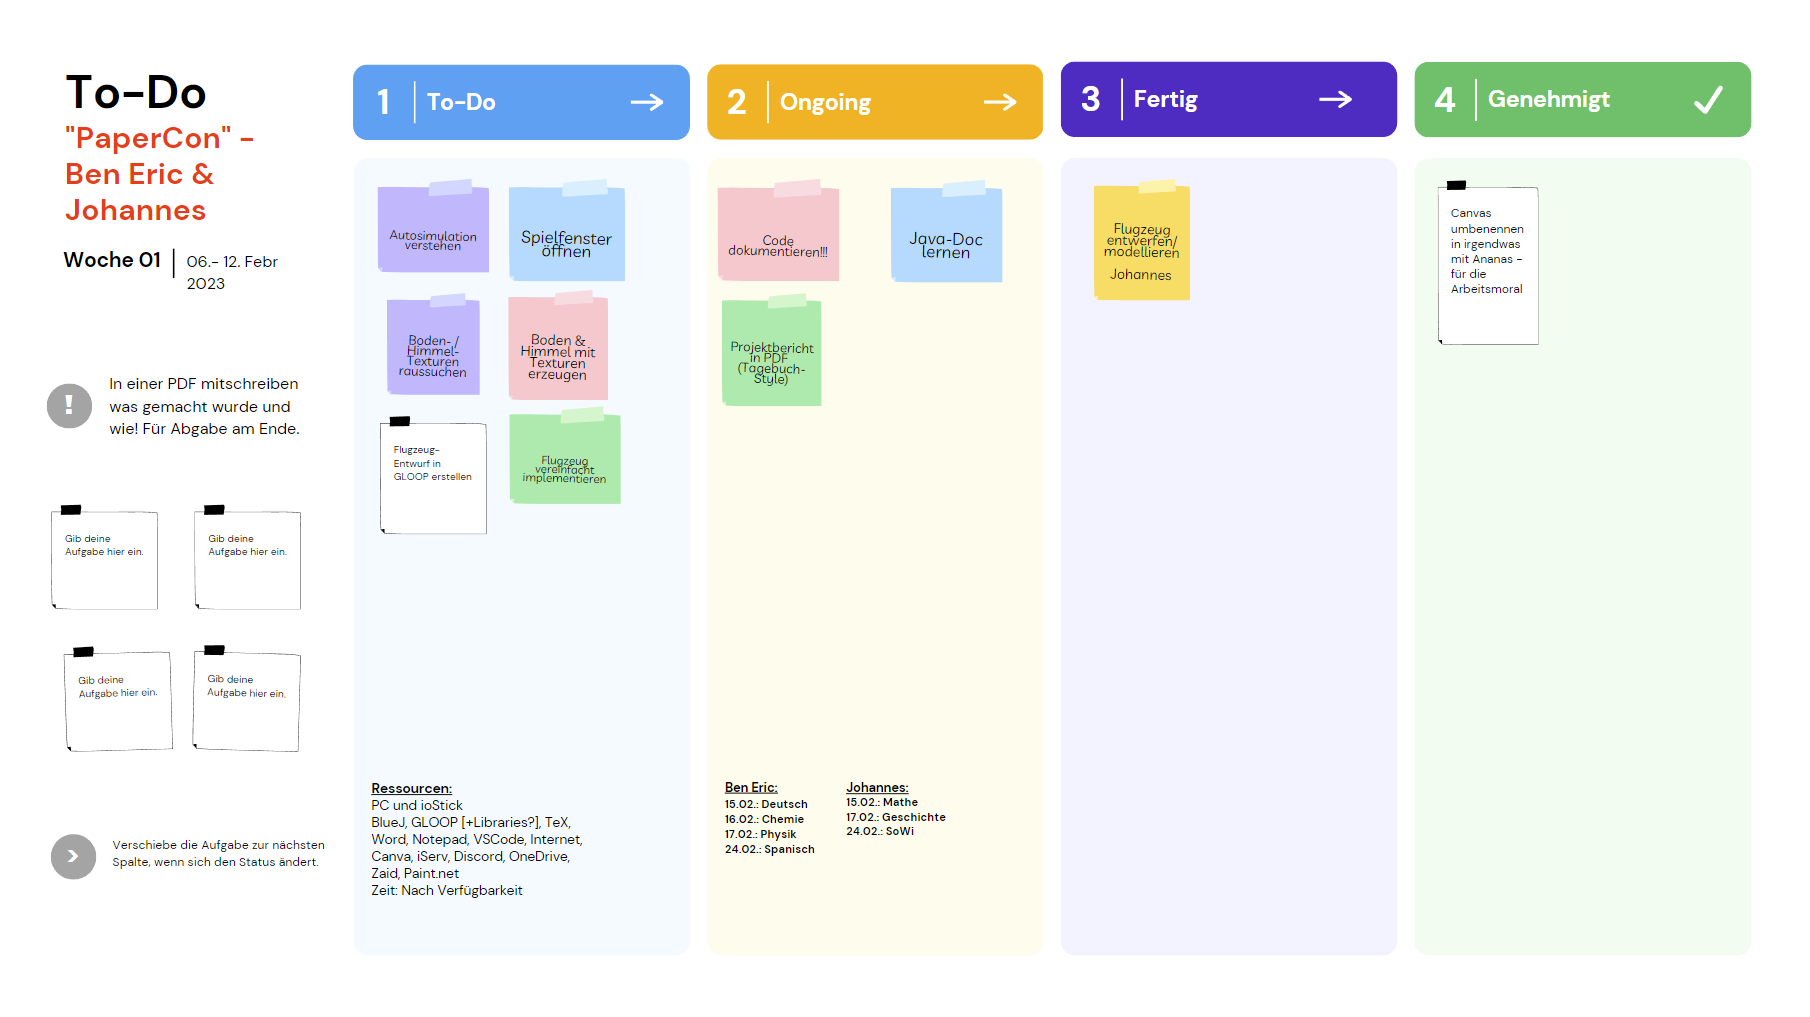
\includegraphics[width=8cm]{Bilder/Canvas/Canva1.png}
%\caption{Flugzeug-Entwurf}
%\end{figure}

\end{spacing}
\end{normalsize}



\section*{14. Februar 2023 - Dienstag:}


\begin{normalsize}
\begin{spacing}{1}

Dieser Tag ist in zwei Arbeitsphasen aufgeteilt: Unterrichtsstunde und Außerhalb der Schule. In den zwanzig Minuten Freiarbeit der Unterrichtstunde war mein Ziel eine Klasse zu erstellen die ein Projektfenster öffnet in welchem später die Objekte abgebildet werden können und teilweise für spätere Objekte die passende Texturen herauszusuchen. Zuhause hatte ich mehrere Ziele. Das erste war die Aufgaben unter IServ zu machen. Die Einleitung ist weiter oben im Dokument zu finden und der aktuelle Stand ist einmal in dem Zip-Ordner der IServ Abgabe oder bei den Canvas zu finden. Die Canvas habe ich auch in der Aufgabe verlinkt. Des weiteren wollte ich den Entwurf des Flugzeugs in GLOOP umsetzen was ich auch geschafft habe (siehe Grafik: Flugzeug-Entwurf).

\begin{figure}[h]
\centering
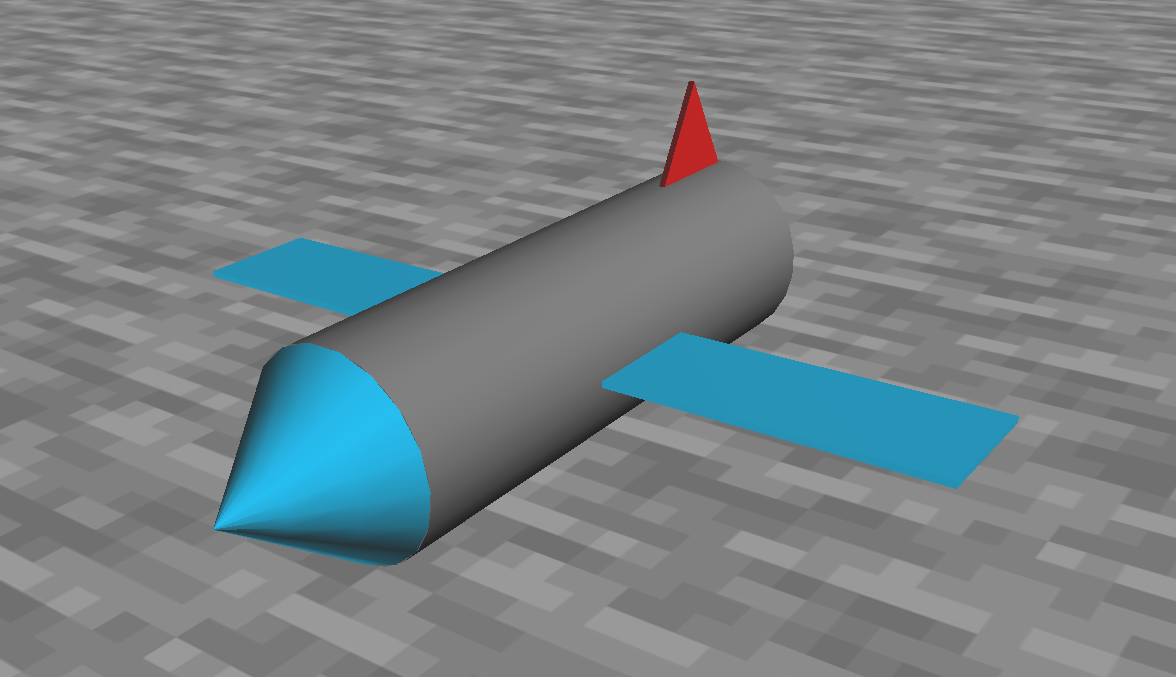
\includegraphics[width=8cm]{Bilder/Screenshots/ScreenshotFlugzeug1.png}
\caption{Flugzeug-Entwurf}
\end{figure}


\end{spacing}
\end{normalsize}
%---------------------------------------------------------------------------------------------------------------------------


\end{document}
